\documentclass[11pt]{amsart}

\usepackage[T1]{fontenc}
\usepackage{lmodern}
\usepackage{amssymb,amsmath}
\usepackage{graphicx}
\usepackage{booktabs}
\usepackage{enumitem}
\usepackage{xcolor}
\usepackage[margin=1.15in]{geometry}
\usepackage[colorlinks=true,linkcolor=blue!50!black,citecolor=blue!50!black,urlcolor=blue!50!black]{hyperref}

\newtheorem{theorem}{Theorem}[section]
\newtheorem{proposition}[theorem]{Proposition}
\newtheorem{lemma}[theorem]{Lemma}
\newtheorem{corollary}[theorem]{Corollary}
\newtheorem*{theoremA}{Theorem A}
\newtheorem*{theoremB}{Theorem B}
\newtheorem*{theoremC}{Theorem C}
\newtheorem*{theoremD}{Theorem D}
\newtheorem*{theoremE}{Theorem E}
\theoremstyle{definition}
\newtheorem{hypothesis}{Hypothesis}
\newtheorem{question}{Question}
\newtheorem{problem}{Problem}
\newtheorem{example}[theorem]{Example}
\theoremstyle{remark}
\newtheorem{remark}[theorem]{Remark}

\numberwithin{equation}{section}

\newcommand{\doi}[1]{\href{https://doi.org/#1}{\nolinkurl{doi:#1}}}
\newcommand{\Ji}{\operatorname{J}}
\newcommand{\Mi}{\operatorname{M}}
\hypersetup{pdftitle={Maximal sublattices of convex geometries: four counterexamples},pdfauthor={Deep Bhattacharjee}}

\begin{document}

\title[Maximal sublattices of convex geometries]{Maximal sublattices of convex geometries:\\ four counterexamples}

\author{Deep Bhattacharjee}
\address{Formerly, Electro-Gravitational Space Propulsion Laboratory (EGSPL),\newline Bhubaneswar, Odisha 751030, India}
\email{d.bhattacharjee@erl-forschung.de}
\email{itsdeep@live.com}
\urladdr{https://orcid.org/0000-0003-0466-750X}
\thanks{Corresponding author: \href{mailto:d.bhattacharjee@erl-forschung.de}{d.bhattacharjee@erl-forschung.de}; ORCID \href{https://orcid.org/0000-0003-0466-750X}{\mbox{0000-0003-0466-750X}}}

\subjclass[2020]{Primary 06B05; Secondary 06B15, 52A01, 05B35}
\keywords{maximal sublattice, convex geometry, join-semidistributive lattice, meet-irreducible element, formal verification}

\begin{abstract}
Adaricheva, Mata, Silberger and Zamojska-Dzienio conjectured that in a finite convex geometry, and more generally in a finite join-semidistributive lattice, the complement of a maximal sublattice is a union of intervals with a common least element, and proved this for convex dimension two. We give convex geometries of convex dimension four and three in which such a complement has two and three minimal elements, so their theorem does not extend. The same examples refute their Hypothesis~4 and one half of their Question~2; an eleven-element convex geometry refutes the other half, and a ten-element lattice their Hypothesis~3.
\end{abstract}

\maketitle

\section{Introduction}

Let $L$ be a finite lattice and $M$ a maximal proper sublattice of $L$, and write $C=L\setminus M$ for its complement. When $L$ is distributive, Chen, Koh and Tan~\cite[Theorem~4]{CKT} and Rival~\cite[Theorem~3]{Ri} showed that $C$ is an interval $[a,b]$ in which $a$ is the only join-irreducible and $b$ the only meet-irreducible element. Adams, Freese, Nation and Schmid~\cite[Theorem~7]{AFNS} proved that $C$ is an interval whenever $L$ is bounded, and asked whether this remains true for finite semidistributive lattices~\cite[p.~7]{AFNS}.

Adaricheva, Mata, Silberger and Zamojska-Dzienio~\cite{AMSZ} took up this question. Since a lattice is semidistributive exactly when it satisfies both the join and the meet semidistributive laws, they also studied the two halves separately, and especially convex geometries, which are join semidistributive. They put forward the following statements~\cite[pp.~2--4 and~25]{AMSZ}, numbered as there.

\begin{hypothesis}\label{h1}
The complements of maximal sublattices of finite semidistributive lattices are intervals.
\end{hypothesis}

\begin{hypothesis}\label{h2}
The complement of a maximal sublattice of a finite convex geometry, or more generally of a finite join-semidistributive lattice, is a union of intervals with a common minimal element.
\end{hypothesis}

\begin{hypothesis}\label{h3}
In every finite lattice the complement of a maximal sublattice is order convex.
\end{hypothesis}

\begin{hypothesis}\label{h4}
If $C$ is the complement of a maximal sublattice $M$ of a finite convex geometry, then every $x\in C$ covers some $m\in M$ with $[0,m]\subseteq M$.
\end{hypothesis}

\setcounter{question}{1}% numbered as in [AMSZ]
\begin{question}\label{q2}
Is it always the case for complements of maximal sublattices of convex geometries that the only join-irreducible element is the minimum and the only meet-irreducible elements are the maxima?
\end{question}

Hypothesis~\ref{h1} is the question of~\cite{AFNS}. Hypothesis~\ref{h2} implies Hypothesis~\ref{h1}, since a semidistributive lattice and its dual are both join semidistributive, and a set that is a union of intervals with a common least element and also with a common greatest element is an interval. Adaricheva et al.\ proved Hypotheses~\ref{h2}, \ref{h3} and~\ref{h4} and gave a positive answer to Question~\ref{q2} for convex geometries of convex dimension two~\cite[Section~6]{AMSZ}. We show that, beyond that case, none of these statements holds in general.

\begin{theoremA}
There is a convex geometry on five points with seventeen closed sets that has a maximal sublattice whose complement has two minimal elements. In this convex geometry Hypotheses~\ref{h2} and~\ref{h4} fail, and so does the first half of Question~\ref{q2}: the complement contains two join-irreducible elements and has no least element.
\end{theoremA}

\begin{theoremB}
There is a convex geometry of convex dimension three on six points with twenty-five closed sets that has a maximal sublattice whose complement has three minimal elements. Hypotheses~\ref{h2} and~\ref{h4} and the first half of Question~\ref{q2} fail in it, so the theorem of Adaricheva et al.\ for convex dimension two does not extend to convex dimension three.
\end{theoremB}

\begin{theoremC}
There is a convex geometry on four points with eleven closed sets that has a maximal sublattice whose complement contains a meet-irreducible element that is not maximal in the complement. So the second half of Question~\ref{q2} fails as well.
\end{theoremC}

\begin{theoremD}
There is a ten-element lattice with a maximal sublattice whose complement is not order convex, so Hypothesis~\ref{h3} fails.
\end{theoremD}

The four examples are given explicitly in Sections~\ref{sec:A}--\ref{sec:D}, with proofs that can be checked by hand. Section~\ref{sec:search} reports the exhaustive computations that located them and shows that they are the smallest of their kind within the ranges searched. In particular no join-semidistributive lattice with at most fourteen elements violates Hypothesis~\ref{h2}; of the $672$ convex geometries on five points exactly six do, the smallest being the one of Theorem~A, and all of them have convex dimension four; and among the convex geometries on six points of convex dimension at most three with at most twenty-five closed sets, the one of Theorem~B is the only one that does.

Hypothesis~\ref{h1} remains open. Our convex geometries are not meet semidistributive (a convex geometry that is meet semidistributive is distributive~\cite{AMSZ}), so they say nothing about it. The computations confirm Hypothesis~\ref{h1} for all semidistributive lattices with at most fourteen elements; by~\cite[Theorem~7]{AFNS} only the lattices that are not bounded matter, and we find exactly one such lattice up to that size, with fourteen elements.

All four examples are also verified in the proof assistant Lean~4~\cite{MU} with Mathlib~\cite{Mathlib}. The formal statements are the negations of the hypotheses themselves, quantified over all finite lattices, with convex geometries described as in~\cite{AMSZ} by join semidistributivity and lower semimodularity. For Theorem~B the formal proof also identifies the lattice with the family of closed sets and shows that three linear orders of the six points realize this family and that no one or two orders do. The proofs use only the standard axioms.

\section{Preliminaries}

All lattices are finite. We write $x\prec y$ when $y$ covers $x$. An element $j\ne0$ is \emph{join-irreducible} if $j=x\vee y$ implies $j\in\{x,y\}$, equivalently if it has exactly one lower cover; \emph{meet-irreducible} elements are defined dually. A lattice is \emph{join semidistributive} if $x\vee y=x\vee z$ implies $x\vee y=x\vee(y\wedge z)$, and \emph{lower semimodular} if $x\prec x\vee y$ implies $x\wedge y\prec y$.

A \emph{convex geometry} on a finite set $X$ is a family $\mathcal G$ of subsets of $X$ that contains $\varnothing$ and $X$, is closed under intersection, and has the anti-exchange property: if $A\in\mathcal G$, $p\ne q$ lie outside $A$, and $q$ lies in the least member of $\mathcal G$ containing $A\cup\{p\}$, then $p$ does not lie in the least member containing $A\cup\{q\}$. Ordered by inclusion, $\mathcal G$ is a lattice with $A\wedge B=A\cap B$ and $A\vee B$ the least member of $\mathcal G$ containing $A\cup B$. A family that contains $\varnothing$ and $X$ and is closed under intersection has the anti-exchange property exactly when every member $A\ne X$ has a one-point extension $A\cup\{x\}$ in the family~\cite{EJ}. Every family obtained by intersecting the initial segments of some linear orders of $X$ is a convex geometry, and every convex geometry arises in this way; the least number of orders needed is the \emph{convex dimension}~\cite{EJ}. The lattices of closed sets of convex geometries are exactly the finite lattices that are join semidistributive and lower semimodular~\cite{AN}; these are Dilworth's meet-distributive lattices~\cite{Di}. Following~\cite{AMSZ} we use the word convex geometry for these lattices as well.

If $M$ is a maximal sublattice of $L$ and $0\notin M$, then $M\cup\{0\}$ is a sublattice, so $C=\{0\}$; dually for $1$. Such complements satisfy all the statements above, and in the examples below $0,1\in M$. To show that a sublattice $M$ is maximal it suffices to show that every sublattice containing $M$ and one element of $C$ is all of $L$.

\section{The convex geometry of Theorem~A}\label{sec:A}

Let $X=\{a,b,c,d,e\}$ and let $\mathcal G_{17}$ consist of the seventeen sets
\begin{equation}\label{eq:G17}
\varnothing,\ a,\ b,\ c,\ d,\ e,\ ac,\ ad,\ bd,\ ae,\ de,\ abd,\ acd,\ ade,\ abde,\ acde,\ abcde,
\end{equation}
where we write $ac$ for $\{a,c\}$ and so on. They are the intersections of the initial segments of the four orders
\[
c<a<d<e<b,\qquad b<d<a<e<c,\qquad a<e<d<c<b,\qquad d<e<a<b<c,
\]
so $\mathcal G_{17}$ is a convex geometry. Directly: $\mathcal G_{17}$ is closed under intersection, and the one-point extensions $\varnothing\subset a\subset ac\subset acd\subset acde\subset X$, $b\subset bd\subset abd\subset abde$, $c\subset ac$, $d\subset ad\subset abd$, $e\subset ae\subset ade\subset abde$ and $de\subset ade$ show that every member other than $X$ has one. Figure~\ref{fig:G17} shows its lattice.

\begin{figure}[ht]
\centering
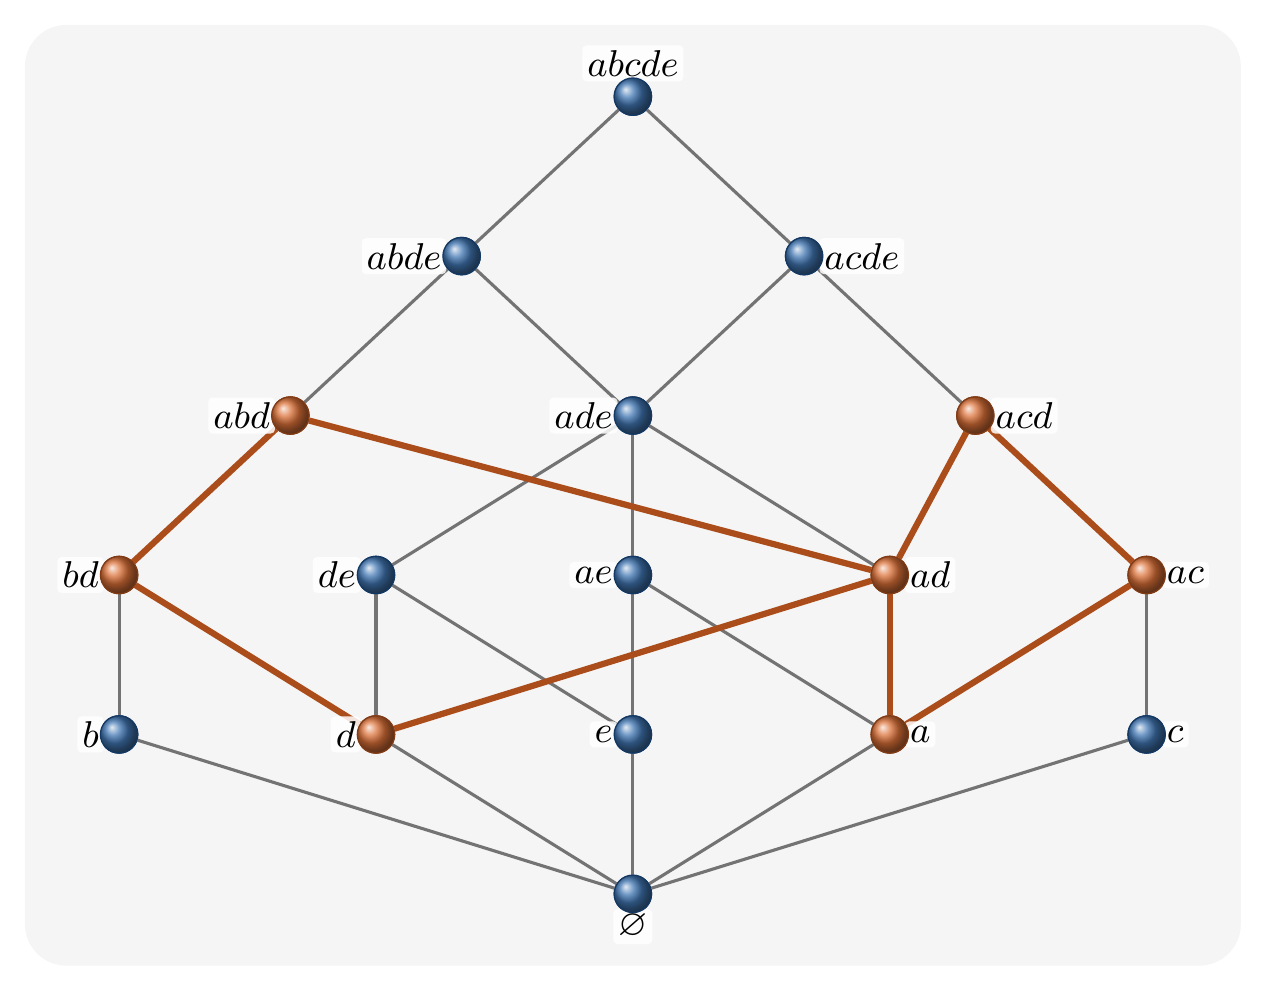
\includegraphics[width=0.66\textwidth]{figures/l17.png}
\caption{The convex geometry $\mathcal G_{17}$. The blue points form the maximal sublattice $M$ of Proposition~\ref{prop:A}, the orange points its complement; the thick edges are the covers inside the complement. Both minimal elements $a$ and $d$ of the complement are atoms.}\label{fig:G17}
\end{figure}

\begin{proposition}\label{prop:A}
Let
\[
M=\{\varnothing,b,c\}\cup\{A\in\mathcal G_{17}:e\in A\}=\{\varnothing,b,c,e,ae,de,ade,abde,acde,X\}.
\]
Then $M$ is a maximal sublattice of $\mathcal G_{17}$, and its complement is
\[
C=\{a,d,ac,ad,bd,abd,acd\}.
\]
\end{proposition}

\begin{proof}
The members containing $e$ form a filter, which is closed under joins and meets. For such a member $A$ the intersections $A\cap b$ and $A\cap c$ are $\varnothing$, $b$ or $c$, and $A\vee b$, $A\vee c$ contain $e$. Finally $b\cap c=\varnothing$, and $b\vee c=X$ because $X$ is the only member containing $b$ and $c$. So $M$ is a sublattice.

Let $S$ be a sublattice that contains $M$ and some $x\in C$. We first show $a\in S$ or $d\in S$. If $x$ is $a$ or $d$ there is nothing to show. Otherwise $x$ is one of $ac$, $ad$, $abd$, $acd$, and then $a=ae\cap x\in S$, or $x=bd$, and then $d=de\cap bd\in S$. Next, if $a\in S$ then $d=de\cap(a\vee b)=de\cap abd\in S$, and if $d\in S$ then $a=ae\cap(c\vee d)=ae\cap acd\in S$. So $a,d\in S$, and then
\[
ac=a\vee c,\quad abd=a\vee b,\quad bd=b\vee d,\quad acd=c\vee d,\quad ad=abd\cap ade
\]
all lie in $S$. Hence $S=\mathcal G_{17}$, and $M$ is maximal.
\end{proof}

\begin{proof}[Proof of Theorem~A]
The complement $C$ of Proposition~\ref{prop:A} has the two minimal elements $a$ and $d$, which are atoms of $\mathcal G_{17}$ and hence join-irreducible. A union of intervals with a common least element has a least element, so Hypothesis~\ref{h2} fails. The element $ad\in C$ covers exactly $a$ and $d$, both outside $M$, so Hypothesis~\ref{h4} fails at $x=ad$. Finally $C$ has no minimum but contains the join-irreducible elements $a$ and $d$, so the first half of Question~\ref{q2} has a negative answer.
\end{proof}

\begin{remark}
The convex dimension of $\mathcal G_{17}$ is four: its meet-irreducible elements $b$, $c$, $ac$, $bd$, $ae$, $de$, $abd$, $acd$, $abde$, $acde$ contain the antichain $\{ac,bd,ae,de\}$, so at least four orders are needed (by the argument of Lemma~\ref{lem:dim} below, or~\cite{EJ}), and four suffice. The complement $C$ is order convex, and in fact every complement of a maximal sublattice of a convex geometry on at most five points is order convex (Section~\ref{sec:search}). Since Adaricheva et al.\ derive the convexity of complements in convex geometries from Hypothesis~\ref{h4}~\cite[Lemma~6.7]{AMSZ}, the restriction of Hypothesis~\ref{h3} to convex geometries is still open.
\end{remark}

\section{The convex geometry of Theorem~B}\label{sec:B}

Let $X=\{a,b,c,d,e,f\}$ and let $\mathcal G_{25}$ consist of the twenty-five sets
\begin{equation}\label{eq:G25}
\begin{gathered}
\varnothing,\ a,\ b,\ c,\ d,\ e,\ f,\ ab,\ bc,\ bd,\ be,\ ce,\ de,\ cf,\ abc,\ bcd,\ bce,\ bde,\ cef,\\ abcd,\ bcde,\ bcef,\ abcde,\ bcdef,\ abcdef.
\end{gathered}
\end{equation}
They are exactly the intersections of the initial segments of the three orders
\begin{equation}\label{eq:orders25}
a<b<c<d<e<f,\qquad f<c<e<b<d<a,\qquad d<e<b<c<a<f,
\end{equation}
so $\mathcal G_{25}$ is a convex geometry; again one can check directly that it is closed under intersection and that every member other than $X$ has a one-point extension. Its lattice is drawn in Figure~\ref{fig:G25}.

\begin{figure}[ht]
\centering
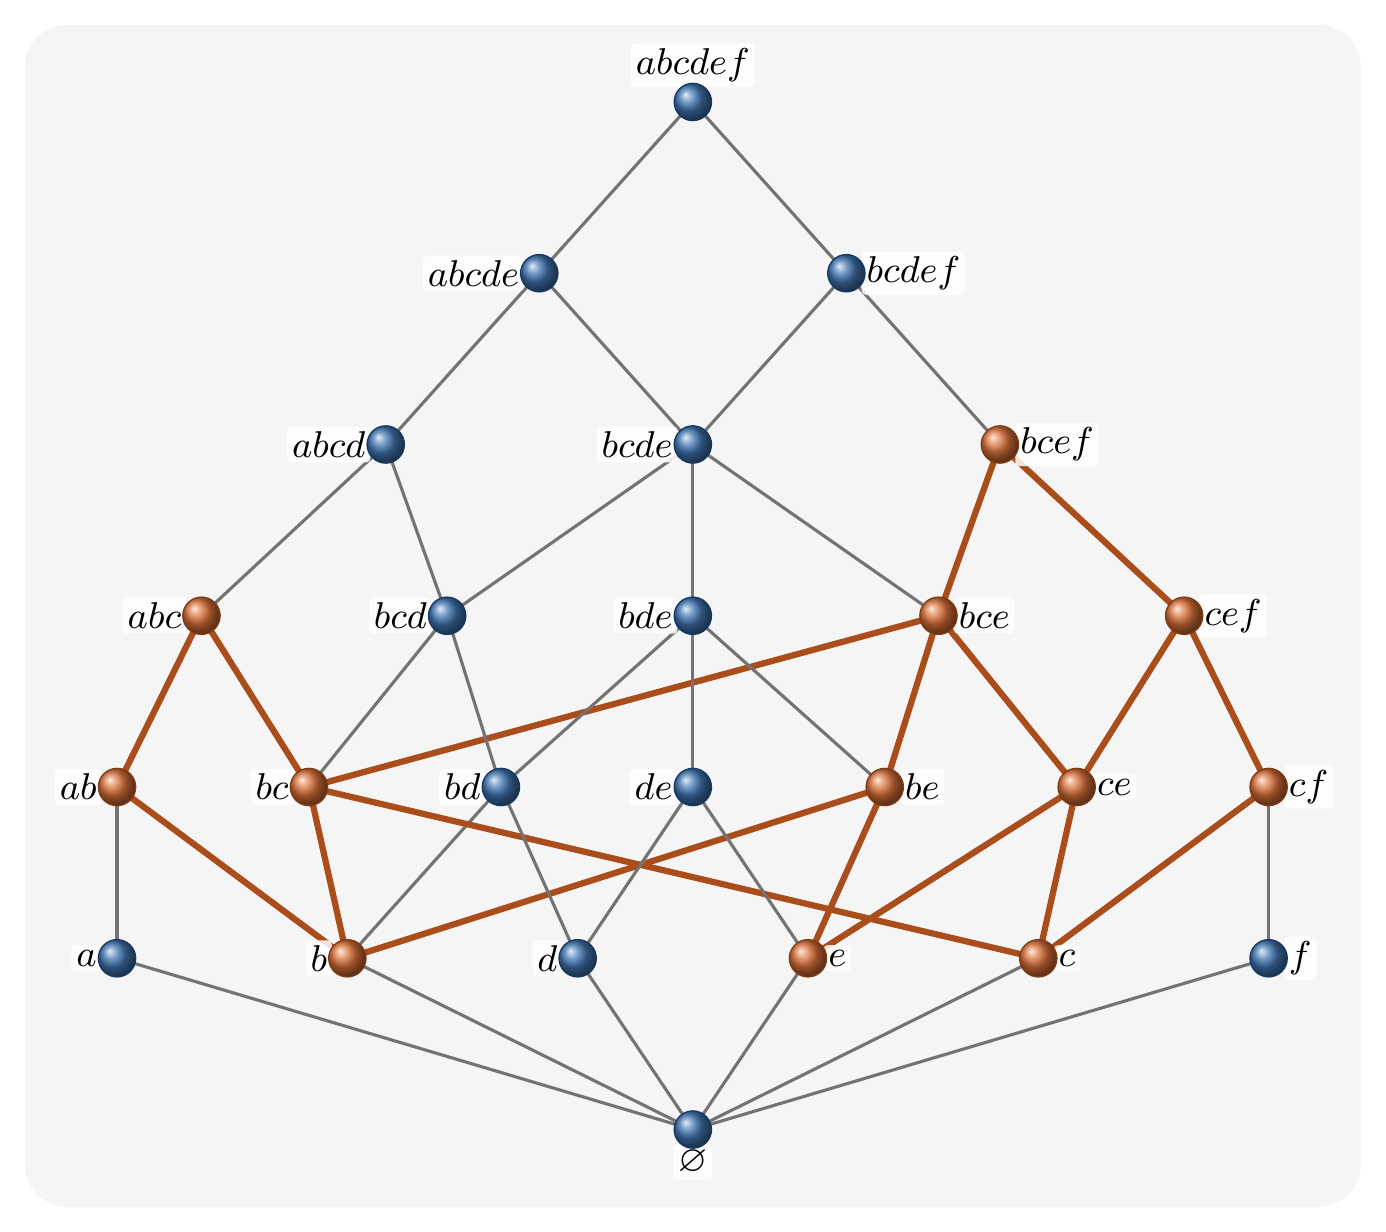
\includegraphics[width=0.8\textwidth]{figures/l25.png}
\caption{The convex geometry $\mathcal G_{25}$ with the maximal sublattice $M$ of Proposition~\ref{prop:B} (blue) and its complement (orange), which has the three minimal elements $b$, $c$ and $e$. The thick edges are the covers inside the complement.}\label{fig:G25}
\end{figure}

\begin{lemma}\label{lem:dim}
The convex dimension of $\mathcal G_{25}$ is three.
\end{lemma}

\begin{proof}
The orders~\eqref{eq:orders25} show that it is at most three. Suppose that the members of $\mathcal G_{25}$ are the intersections of the initial segments of some linear orders. Every initial segment is then a member, and every member $K\ne X$ is the intersection of the least initial segments of each order that contain it. If $K$ is meet-irreducible, it is therefore one of these initial segments. The sets $ab$, $de$ and $cf$ are meet-irreducible, with the single upper covers $abc$, $bde$ and $cef$, and no two of them are comparable; since the initial segments of one order form a chain, they are initial segments of three different orders.
\end{proof}

The argument is the easy half of the theorem of Edelman and Jamison that the convex dimension is the width of the poset of meet-irreducible closed sets~\cite{EJ}.

\begin{proposition}\label{prop:B}
Let
\[
M=\{\varnothing,a,f\}\cup\{A\in\mathcal G_{25}:d\in A\}=\{\varnothing,a,d,f,bd,de,bcd,bde,abcd,bcde,abcde,bcdef,X\}.
\]
Then $M$ is a maximal sublattice of $\mathcal G_{25}$, and its complement is
\[
C=\{b,c,e,ab,bc,be,ce,cf,abc,bce,cef,bcef\}.
\]
\end{proposition}

\begin{proof}
As in Proposition~\ref{prop:A}, the members containing $d$ form a filter; for such a member $A$ the intersections $A\cap a$ and $A\cap f$ lie in $\{\varnothing,a,f\}$ and $A\vee a$, $A\vee f$ contain $d$; and $a\cap f=\varnothing$, $a\vee f=X$, because $X$ is the only member containing $a$ and $f$. So $M$ is a sublattice.

Let $S$ be a sublattice that contains $M$ and some $x\in C$. First, $S$ contains one of $b$, $c$, $e$: if $x$ is one of $ab$, $bc$, $be$, $abc$, $bce$, $bcef$ then $b=x\cap bd$; if $x=ce$ then $e=ce\cap de$; and if $x$ is $cf$ or $cef$ then $c=x\cap bcd$. Next,
\[
b\in S\Rightarrow e=(b\vee f)\cap de=bcef\cap de\in S,\qquad e\in S\Rightarrow c=(e\vee f)\cap bcd=cef\cap bcd\in S,
\]
\[
c\in S\Rightarrow b=(a\vee c)\cap bd=abc\cap bd\in S,
\]
so $b,c,e\in S$. Finally
\begin{gather*}
ab=a\vee b,\quad bc=b\vee c,\quad be=b\vee e,\quad ce=c\vee e,\quad cf=c\vee f,\\ abc=a\vee c,\quad bce=bc\vee e,\quad cef=e\vee f,\quad bcef=b\vee f
\end{gather*}
lie in $S$, and $S=\mathcal G_{25}$.
\end{proof}

\begin{proof}[Proof of Theorem~B]
By Lemma~\ref{lem:dim} the convex dimension of $\mathcal G_{25}$ is three. The complement $C$ of Proposition~\ref{prop:B} has the three minimal elements $b$, $c$ and $e$, all atoms, so it has no least element and Hypothesis~\ref{h2} fails. The element $bc\in C$ covers exactly $b$ and $c$, so Hypothesis~\ref{h4} fails at $x=bc$, and the join-irreducible elements $b$, $c$, $e$ of $C$ show that the first half of Question~\ref{q2} fails as well.
\end{proof}

\begin{remark}
In $\mathcal G_{17}$ and in $\mathcal G_{25}$ the maximal sublattice consists of the least element, two atoms whose join is the greatest element, and the filter generated by a third atom. The complement of $M$ in $\mathcal G_{25}$ is again order convex: none of its members contains $d$, while every member of $M$ other than $\varnothing$, $a$ and $f$ does.
\end{remark}

\section{The convex geometry of Theorem~C}\label{sec:C}

Let $X=\{a,b,c,d\}$ and let $\mathcal G_{11}$ consist of
\[
\varnothing,\ a,\ b,\ c,\ ab,\ ac,\ ad,\ bc,\ abc,\ abd,\ abcd,
\]
the intersections of the initial segments of the orders $a<c<b<d$, $a<d<b<c$ and $b<c<a<d$. It is closed under intersection, and $\varnothing\subset a\subset ab\subset abc\subset X$, $b\subset bc\subset abc$, $c\subset ac\subset abc$, $ad\subset abd\subset X$ are one-point extensions of all its members, so it is a convex geometry, of convex dimension three. Its lattice is drawn in Figure~\ref{fig:G11}.

\begin{figure}[ht]
\centering
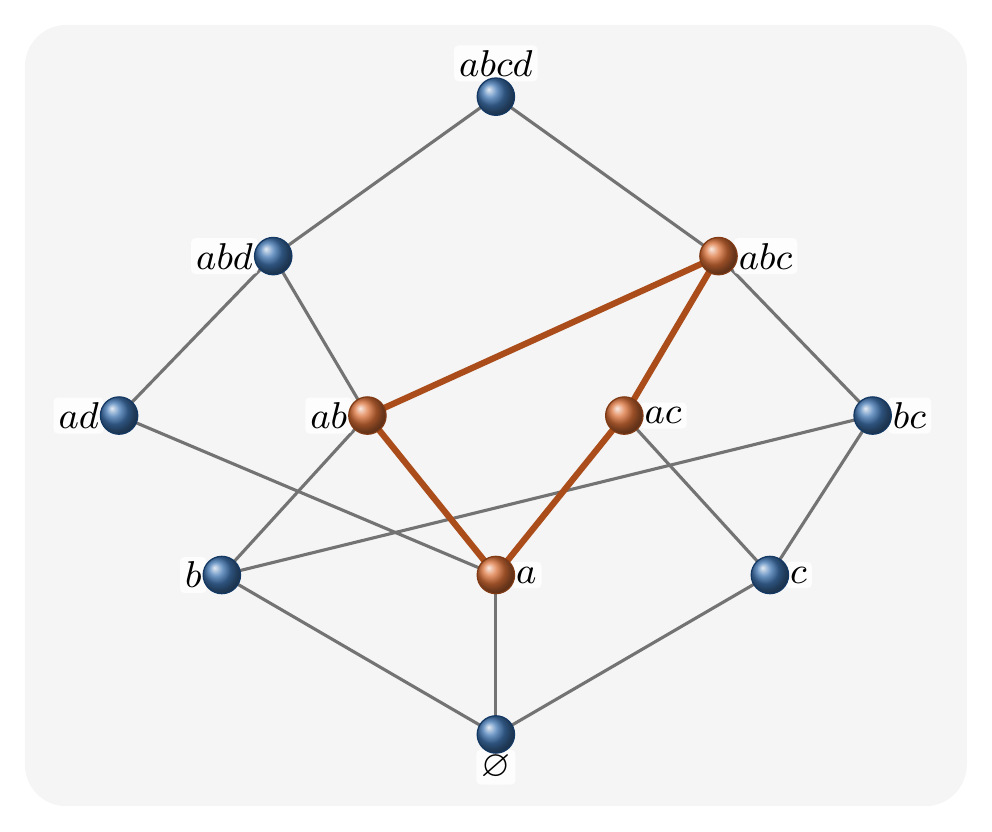
\includegraphics[width=0.52\textwidth]{figures/l11.png}
\caption{The convex geometry $\mathcal G_{11}$ with the maximal sublattice $M$ of Proposition~\ref{prop:C} (blue) and its complement $[a,abc]$ (orange).}\label{fig:G11}
\end{figure}

\begin{proposition}\label{prop:C}
The set $M=\{\varnothing,b,c,bc,ad,abd,X\}$ is a maximal sublattice of $\mathcal G_{11}$, with complement the interval $C=[a,abc]=\{a,ab,ac,abc\}$. The element $ac$ is meet-irreducible and lies below $abc\in C$.
\end{proposition}

\begin{proof}
The members not containing $a$ are $\varnothing,b,c,bc$; they are closed under intersection, and $b\vee c=bc$. A join of one of $b,c,bc$ with $ad$ or $abd$ is $abd$ if it does not contain $c$, and $X$ if it does, because $X$ is the only member containing $a$, $c$ and $d$; meets give $ad\cap b=ad\cap c=ad\cap bc=\varnothing$, $abd\cap b=abd\cap bc=b$ and $abd\cap c=\varnothing$. So $M$ is a sublattice. If a sublattice $S$ contains $M$ and some $x\in C$, then $a=ad\cap x\in S$, hence $ab=a\vee b$, $ac=a\vee c$ and $abc=ab\vee c$ lie in $S$, and $S=\mathcal G_{11}$. The only member strictly between $ac$ and $X$ is $abc$, so $ac$ has the single upper cover $abc$.
\end{proof}

Theorem~C follows: $ac$ is a meet-irreducible element of $C$ that is not a maximal element of $C$. Here $C$ is an interval and its only join-irreducible element is its minimum $a$, so $\mathcal G_{11}$ satisfies Hypotheses~\ref{h2} and~\ref{h4}; the failure of Question~\ref{q2} is independent of the failure of Hypothesis~\ref{h2}.

\section{The lattice of Theorem~D}\label{sec:D}

Let $L_{10}=\{0,1,\dots,9\}$ be the lattice with covering pairs
\begin{gather*}
0\prec1,\ 0\prec2,\ 0\prec3,\ 1\prec8,\ 2\prec5,\ 2\prec6,\ 3\prec4,\\ 3\prec5,\ 4\prec9,\ 5\prec7,\ 5\prec8,\ 6\prec7,\ 7\prec9,\ 8\prec9,
\end{gather*}
drawn in Figure~\ref{fig:L10}.

\begin{figure}[ht]
\centering
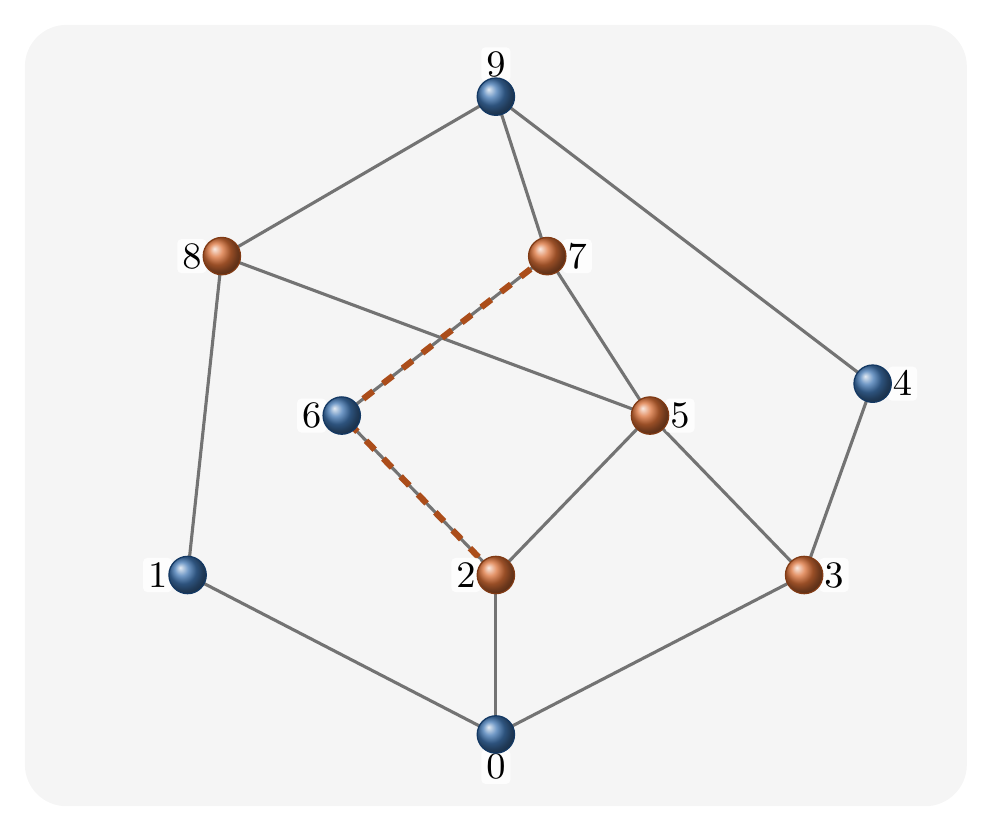
\includegraphics[width=0.52\textwidth]{figures/l10.png}
\caption{The lattice $L_{10}$. The blue points form a maximal sublattice isomorphic to $M_3$; the orange points form its complement, which contains $2<7$ but not $6$ (dashed).}\label{fig:L10}
\end{figure}

\begin{proposition}\label{prop:D}
The set $M=\{0,1,4,6,9\}$ is a maximal sublattice of $L_{10}$, isomorphic to the five-element modular lattice $M_3$. Its complement $\{2,3,5,7,8\}$ contains $2$ and $7$ but not $6$, although $2<6<7$.
\end{proposition}

\begin{proof}
Any two of $1,4,6$ have join $9$ and meet $0$, so $M$ is a sublattice isomorphic to $M_3$. Let $S$ be a sublattice containing $M$ and one of $2,3,5,7,8$. The following identities show that $S$ then contains all of $L_{10}$:
\begin{align*}
2:&\quad 8=1\vee2,\ 3=4\wedge8,\ 7=6\vee3,\ 5=2\vee3;\\
3:&\quad 8=1\vee3,\ 7=6\vee3,\ 2=6\wedge8,\ 5=2\vee3;\\
5:&\quad 8=1\vee5,\ 3=4\wedge5,\ 7=6\vee5,\ 2=6\wedge5;\\
7:&\quad 3=4\wedge7,\ 8=1\vee3,\ 2=6\wedge8,\ 5=7\wedge8;\\
8:&\quad 3=4\wedge8,\ 2=6\wedge8,\ 7=6\vee3,\ 5=7\wedge8.
\end{align*}
Each identity is read off the covering relation; for instance $1\vee2=8$ because $8$ and $9$ are the only common upper bounds of $1$ and $2$, and $4\wedge8=3$ because $0$ and $3$ are the only common lower bounds of $4$ and $8$.
\end{proof}

Theorem~D follows. Adams, Freese, Nation and Schmid~\cite[Figure~1]{AFNS} drew an infinite lattice with a maximal sublattice isomorphic to $M_3$ and noted that an obvious modification gives finite lattices with the same property. We have not determined whether the complements in those lattices are order convex; $L_{10}$ is the smallest lattice in which the complement of a maximal sublattice is not.

\section{Computations}\label{sec:search}

The examples were found by two exhaustive searches.

\emph{All lattices with at most fourteen elements.} The program \texttt{nauty-genposetg} of Brinkmann and McKay~\cite{BM,MP} lists the posets on $n$ points up to isomorphism; adding a least and a greatest element and keeping the lattices gives every lattice with $n+2$ elements once. For each lattice our C program finds all maximal sublattices by running through all subsets, and tests Hypotheses~\ref{h1}--\ref{h4} and both halves of Question~\ref{q2}. For fourteen elements it treats the $1{,}104{,}891{,}746$ posets on twelve points and keeps the lattices that are join or meet semidistributive. A second program, written independently in Python, repeats the convexity test for all lattices with at most ten elements and the tests of Question~\ref{q2} for all convex geometries with at most eleven elements. The lattice counts agree with the sequence A006966 of~\cite{OEIS}.

\begin{table}[ht]
\centering
\small
\begin{tabular}{rrrrrrrr}
\toprule
$|L|$ & lattices & SD$_\vee$ & SD & CG & non-convex & Q2, meet half & H1, H2, H4, Q2 join half \\
\midrule
2--9 & $1{,}377$ & $302$ & $273$ & $70$ & $0$ & $0$ & $0$\\
10 & $5{,}994$ & $636$ & $534$ & $62$ & $1$ & $0$ & $0$\\
11 & $37{,}622$ & $2{,}171$ & $1{,}720$ & $121$ & $15$ & $1$ & $0$\\
12 & $262{,}776$ & $7{,}756$ & $5{,}767$ & $244$ & $167$ & $3$ & $0$\\
13 & $2{,}018{,}305$ & $28{,}822$ & $20{,}013$ & $497$ & -- & $12$ & $0$\\
14 & $16{,}873{,}364$ & $110{,}805$ & $71{,}546$ & $1{,}031$ & -- & $33$ & $0$\\
\bottomrule
\end{tabular}
\caption{Lattices $L$ by size: all lattices, the join-semidistributive (SD$_\vee$) and semidistributive (SD) ones, and convex geometries (CG); then the number of maximal sublattices whose complement is not order convex (over all lattices, computed up to twelve elements), the number of maximal sublattices of convex geometries violating the second half of Question~\ref{q2}, and the number violating Hypotheses~\ref{h1}, \ref{h2}, \ref{h4} or the first half of Question~\ref{q2} in the classes where they are stated. In join- or meet-semidistributive lattices with at most fourteen elements every complement is order convex.}\label{tab:counts}
\end{table}

\begin{theoremE}
\begin{enumerate}[label=\textup{(\roman*)},leftmargin=*]
\item Every join-semidistributive lattice with at most fourteen elements satisfies Hypothesis~\ref{h2}, and every semidistributive one satisfies Hypothesis~\ref{h1}.
\item No lattice with at most nine elements has a maximal sublattice with a complement that is not order convex, and $L_{10}$ is the only such lattice with ten elements.
\item No convex geometry with at most ten elements violates the second half of Question~\ref{q2}, and $\mathcal G_{11}$ is the only one with eleven elements.
\item Every convex geometry on at most four points satisfies Hypotheses~\ref{h2} and~\ref{h4} and the first half of Question~\ref{q2}. Of the $672$ convex geometries on five points exactly six violate Hypothesis~\ref{h2}; they have $17$, $18$, $19$, $19$, $20$ and $21$ closed sets, all have convex dimension four, and the smallest is $\mathcal G_{17}$. In each of them the same complement also violates Hypothesis~\ref{h4} and the first half of Question~\ref{q2}, and no other complement does.
\item Up to isomorphism there are $8{,}435$ convex geometries on six points of convex dimension at most three with at most $25$ closed sets, and $\mathcal G_{25}$ is the only one of them that violates Hypothesis~\ref{h2}.
\end{enumerate}
\end{theoremE}

For part~(iv) the convex geometries on five points were generated directly: a search through families of subsets of $X$, closed under intersection and with one-point extensions, produced the $59{,}386$ labelled and $672$ unlabelled geometries, in agreement with the known counts. The maximal sublattices were found with a SAT solver~\cite{IMM}: a model of the clauses saying that a set of elements is closed under joins and meets, contains $0$ and $1$ and is proper is extended greedily to a maximal sublattice, which is then excluded, until no model remains. The $597$ geometries with at most $22$ closed sets were checked again by the C program. For part~(v) we ran through all pairs of linear orders of six points, with a fixed first order, formed the intersections of the initial segments of the three orders, and kept the $56{,}990$ families with at most $25$ members; they fall into $8{,}435$ isomorphism classes, whose maximal sublattices we found in the same way. Up to fourteen elements there is exactly one semidistributive lattice that is not bounded; it has fourteen elements, and its six maximal sublattices have intervals as complements.

\section{Questions}

Hypothesis~\ref{h2} holds in convex dimension two~\cite{AMSZ} and fails in convex dimension three. By Theorem~E a counterexample of convex dimension three has more than fourteen elements and at least six points, and $\mathcal G_{25}$ is the smallest one on six points.

\begin{problem}
What is the least number of closed sets of a convex geometry of convex dimension three that violates Hypothesis~\ref{h2}?
\end{problem}

\begin{problem}
Is the complement of a maximal sublattice of a finite convex geometry always order convex?
\end{problem}

The main question, Hypothesis~\ref{h1}, is untouched by the examples above: a counterexample would have to be semidistributive and not bounded, and Theorem~E shows it would have more than fourteen elements.

\subsection*{Data availability}
The Lean~4 development, the programs of Section~\ref{sec:search} and their outputs are archived with the source of this paper~\cite{Ar}.

\subsection*{Use of generative AI}
During the preparation of this work the author used Claude (Anthropic) to search the literature, to run and check the computations and the formal proofs, and to draft the text. The author checked every step of the proofs and every reference, and takes full responsibility for the content.

\begin{thebibliography}{99}

\bibitem{AFNS}
M.~E.~Adams, R.~Freese, J.~B.~Nation and J.~Schmid, \emph{Maximal sublattices and Frattini sublattices of bounded lattices}, J. Austral. Math. Soc. Ser.~A \textbf{63} (1997), 110--127. \doi{10.1017/S1446788700000355}

\bibitem{AMSZ}
K.~Adaricheva, A.~Mata, S.~Silberger and A.~Zamojska-Dzienio, \emph{Conjecture on maximal sublattices of finite semidistributive lattices and beyond}, Discrete Math. Theor. Comput. Sci. \textbf{28}:2 (2026). \doi{10.46298/dmtcs.16374}

\bibitem{AN}
K.~Adaricheva and J.~B.~Nation, \emph{Convex geometries}, in: G.~Gr\"atzer and F.~Wehrung (eds.), Lattice Theory: Special Topics and Applications, Vol.~2, Birkh\"auser, Cham, 2016, 153--179. \doi{10.1007/978-3-319-44236-5_5}

\bibitem{Ar}
D.~Bhattacharjee, \emph{Maximal sublattices of convex geometries: paper, Lean~4 development and computations}, 2026. \url{https://github.com/creelie/congenial-robot}

\bibitem{BM}
G.~Brinkmann and B.~D.~McKay, \emph{Posets on up to 16 points}, Order \textbf{19} (2002), 147--179. \doi{10.1023/A:1016543307592}

\bibitem{CKT}
C.~C.~Chen, K.~M.~Koh and S.~K.~Tan, \emph{Frattini sublattices of distributive lattices}, Algebra Universalis \textbf{3} (1973), 294--303. \doi{10.1007/BF02945131}

\bibitem{Di}
R.~P.~Dilworth, \emph{Lattices with unique irreducible decompositions}, Ann. of Math. (2) \textbf{41} (1940), 771--777. \doi{10.2307/1968857}

\bibitem{EJ}
P.~H.~Edelman and R.~E.~Jamison, \emph{The theory of convex geometries}, Geom. Dedicata \textbf{19} (1985), 247--270. \doi{10.1007/BF00149365}

\bibitem{IMM}
A.~Ignatiev, A.~Morgado and J.~Marques-Silva, \emph{PySAT: a Python toolkit for prototyping with SAT oracles}, in: Theory and Applications of Satisfiability Testing (SAT 2018), Lecture Notes in Comput. Sci. \textbf{10929}, Springer, Cham, 2018, 428--437. \doi{10.1007/978-3-319-94144-8_26}

\bibitem{Mathlib}
The mathlib Community, \emph{The Lean mathematical library}, in: Proceedings of the 9th ACM SIGPLAN International Conference on Certified Programs and Proofs (CPP 2020), ACM, New York, 2020, 367--381. \doi{10.1145/3372885.3373824}

\bibitem{MP}
B.~D.~McKay and A.~Piperno, \emph{Practical graph isomorphism, II}, J. Symbolic Comput. \textbf{60} (2014), 94--112. \doi{10.1016/j.jsc.2013.09.003}

\bibitem{MU}
L.~de~Moura and S.~Ullrich, \emph{The Lean~4 theorem prover and programming language}, in: Automated Deduction -- CADE~28, Lecture Notes in Comput. Sci. \textbf{12699}, Springer, Cham, 2021, 625--635. \doi{10.1007/978-3-030-79876-5_37}

\bibitem{OEIS}
OEIS Foundation Inc., \emph{The On-Line Encyclopedia of Integer Sequences}, sequence A006966 (number of lattices on $n$ unlabeled nodes). \url{https://oeis.org/A006966}

\bibitem{Ri}
I.~Rival, \emph{Maximal sublattices of finite distributive lattices}, Proc. Amer. Math. Soc. \textbf{37} (1973), 417--420. \doi{10.1090/S0002-9939-1973-0311527-9}

\end{thebibliography}

\end{document}
